% auto-generated — figures in ../figures/appendix/（subcaption で横並び）
\begin{figure}[!htbp]
  \centering
  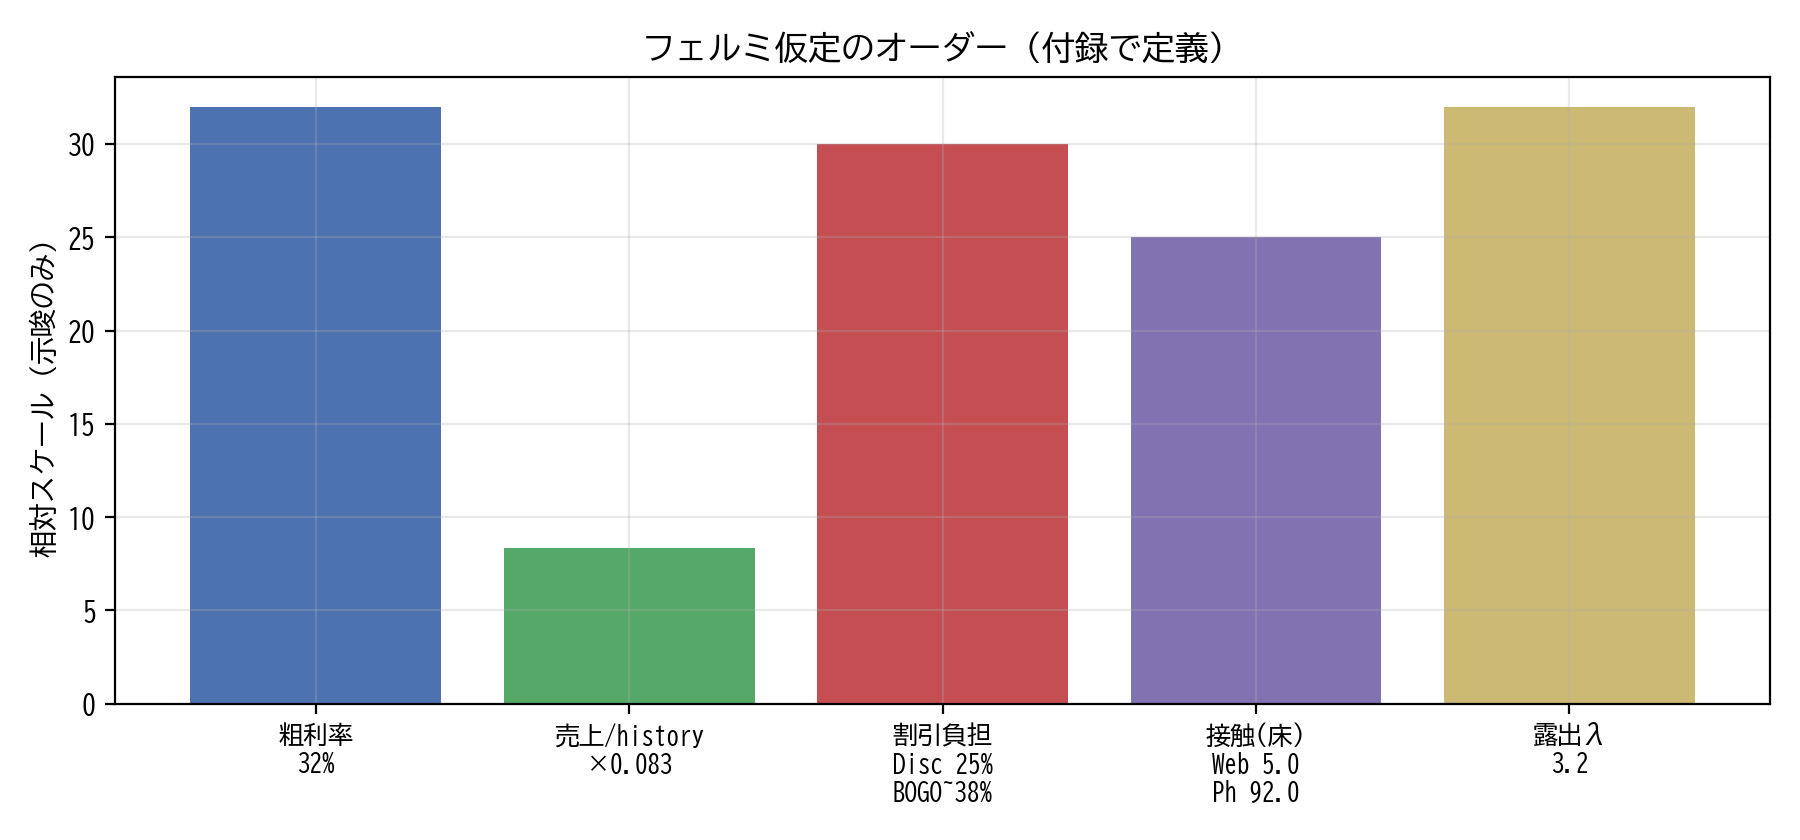
\includegraphics[width=0.88\linewidth]{../figures/appendix/fig_fermi_schematic.png}
  \caption{フェルミ仮定のオーダー（粗利・売上スケール・オファー負担・接触・露出）。}
  \label{fig:app-fermi-schematic}
\end{figure}

\begin{figure}[!htbp]
  \centering
  \begin{subfigure}[t]{0.49\linewidth}
    \centering
    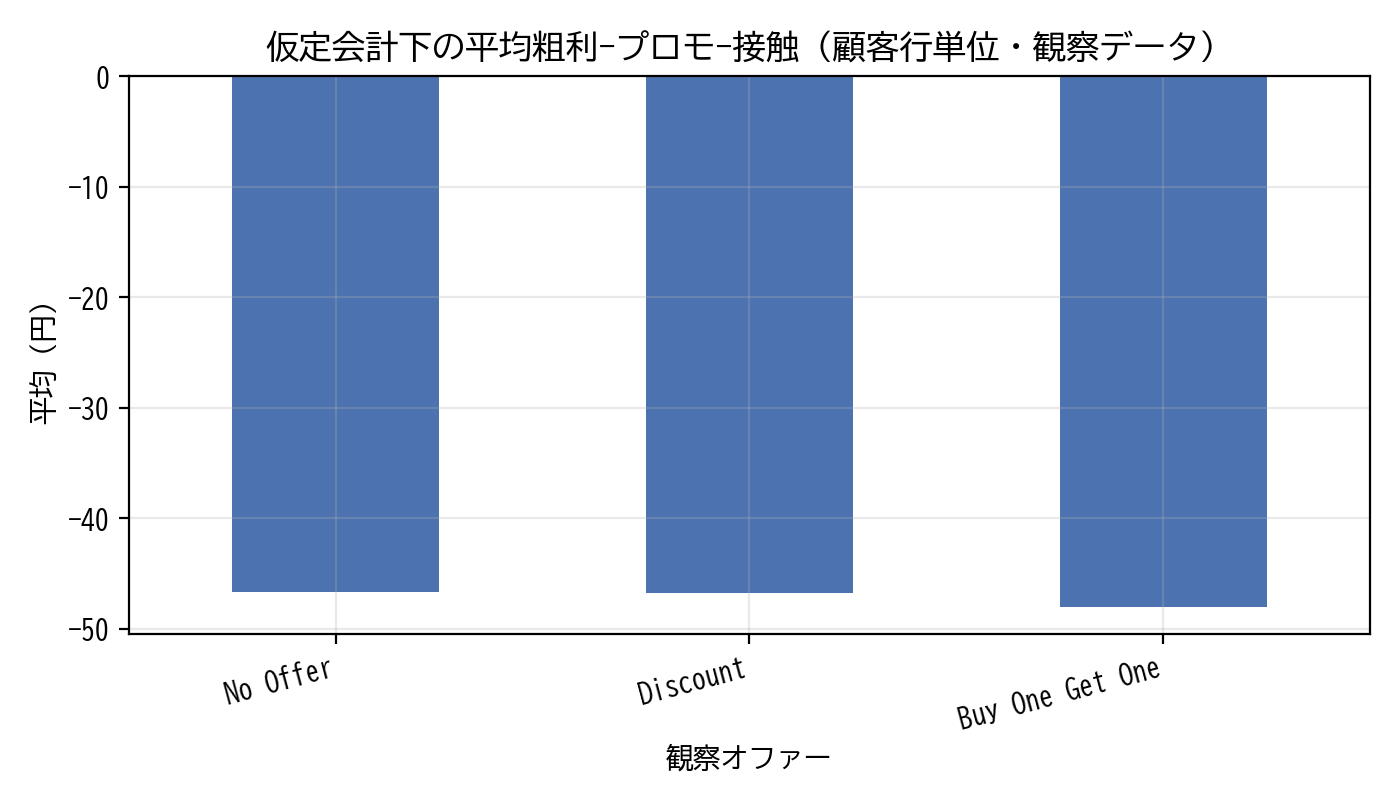
\includegraphics[width=\linewidth]{../figures/appendix/fig_profit_by_observed_offer.png}
    \caption{観察オファー別の平均利益（粗利−プロモ−接触）。因果効果ではない。}
    \label{fig:app-profit-offer}
  \end{subfigure}\hfill
  \begin{subfigure}[t]{0.49\linewidth}
    \centering
    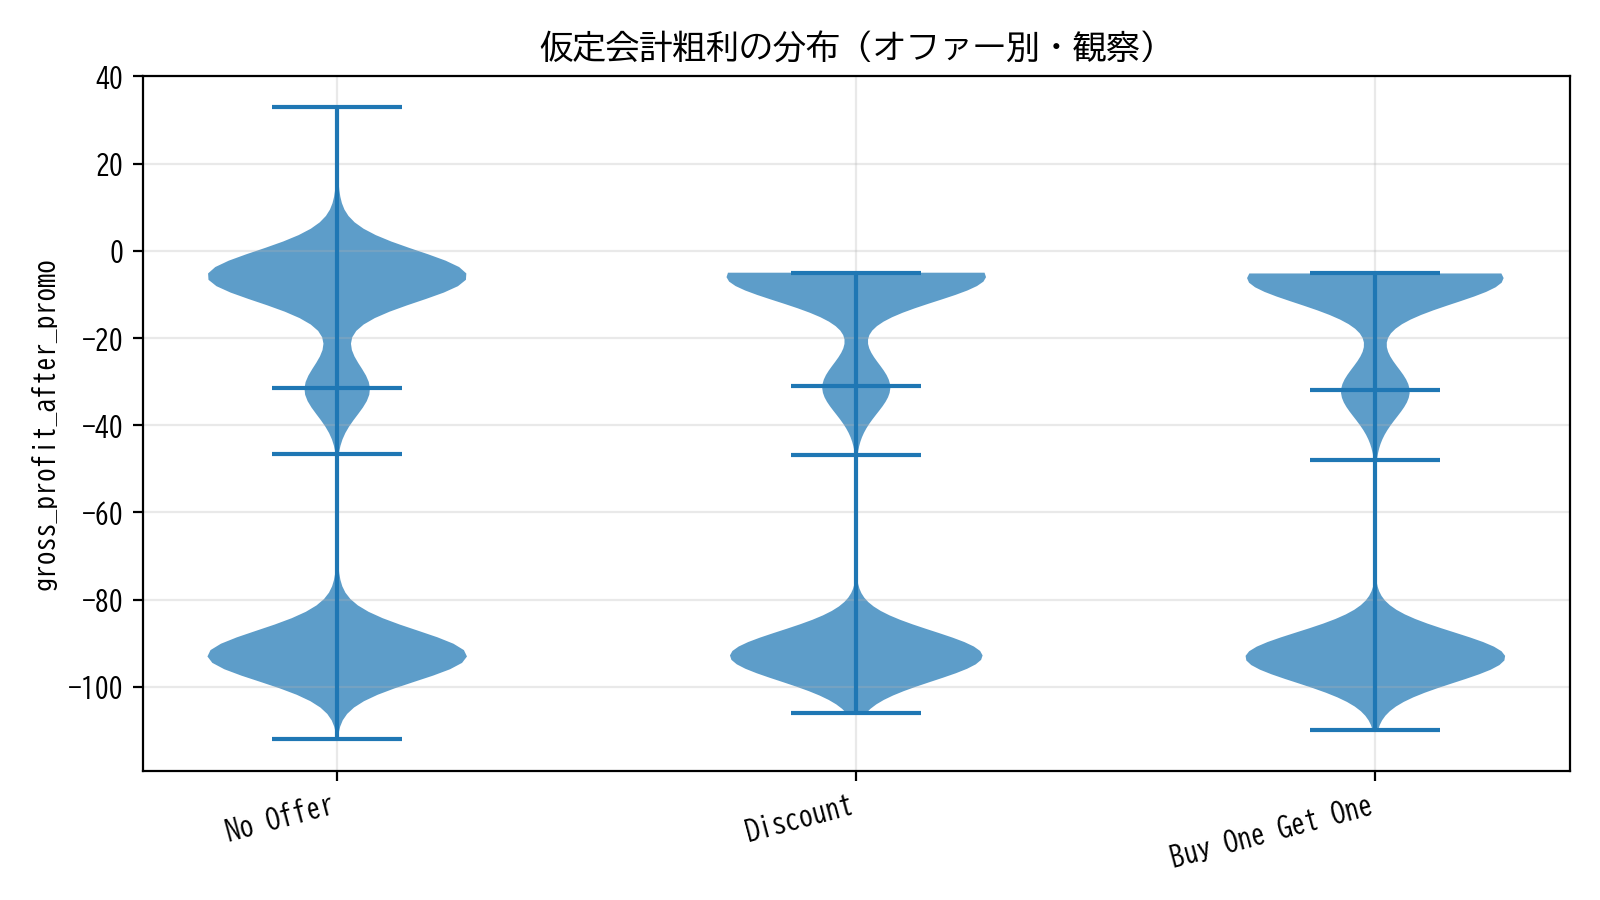
\includegraphics[width=\linewidth]{../figures/appendix/fig_gp_violin_by_offer.png}
    \caption{同・仮定会計での利益分布（バイオリン）。}
    \label{fig:app-gp-violin}
  \end{subfigure}
  \caption{仮定会計におけるオファー別の水準と分布}
\end{figure}

\begin{figure}[!htbp]
  \centering
  \begin{subfigure}[t]{0.49\linewidth}
    \centering
    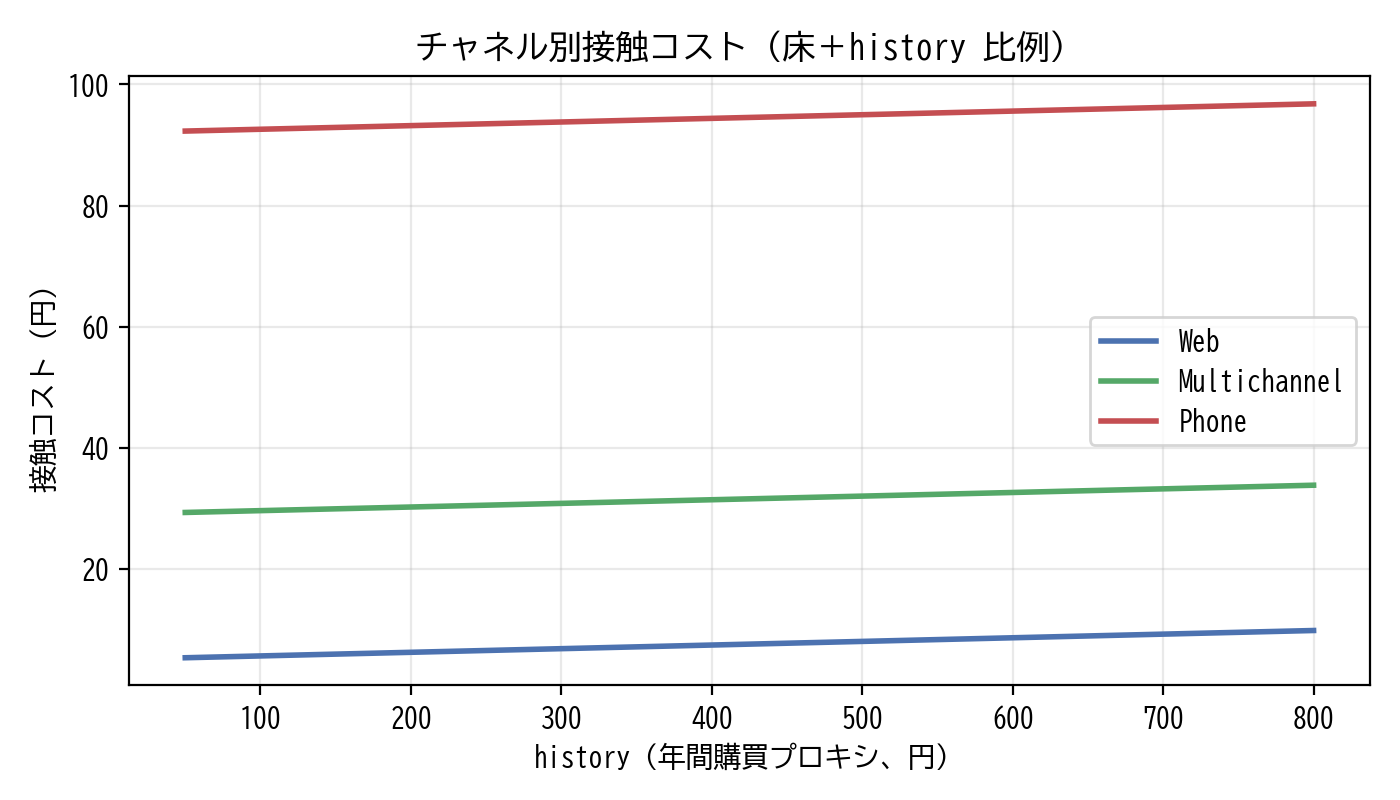
\includegraphics[width=\linewidth]{../figures/appendix/fig_contact_cost_by_channel.png}
    \caption{チャネル別の接触コスト曲線（床＋history比例）。}
    \label{fig:app-contact}
  \end{subfigure}\hfill
  \begin{subfigure}[t]{0.49\linewidth}
    \centering
    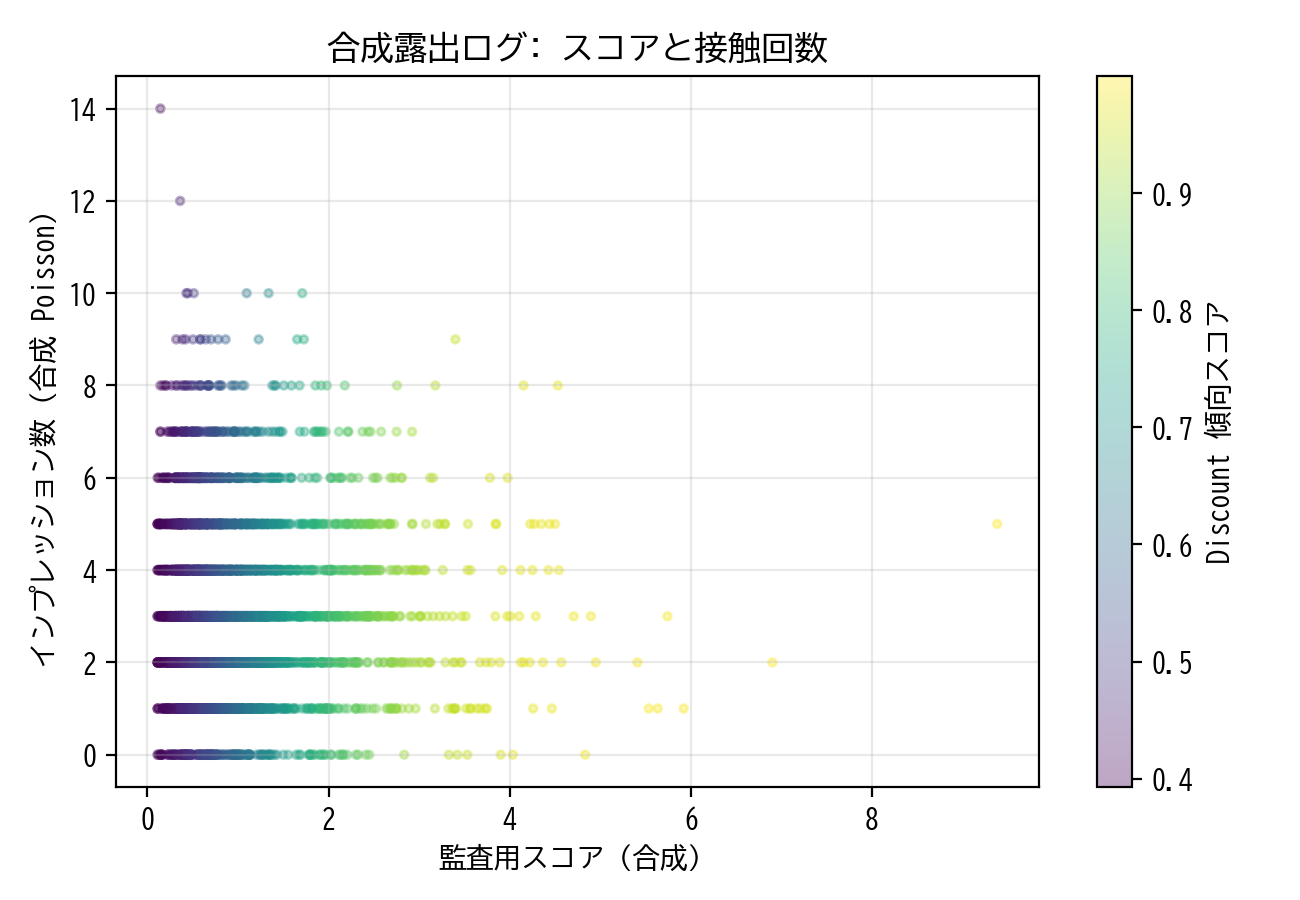
\includegraphics[width=\linewidth]{../figures/appendix/fig_exposure_scatter_audit.png}
    \caption{合成露出ログ：監査スコアとインプレッション数。}
    \label{fig:app-exposure}
  \end{subfigure}
  \caption{接触コストと合成露出}
\end{figure}

\begin{figure}[!htbp]
  \centering
  \begin{subfigure}[t]{0.49\linewidth}
    \centering
    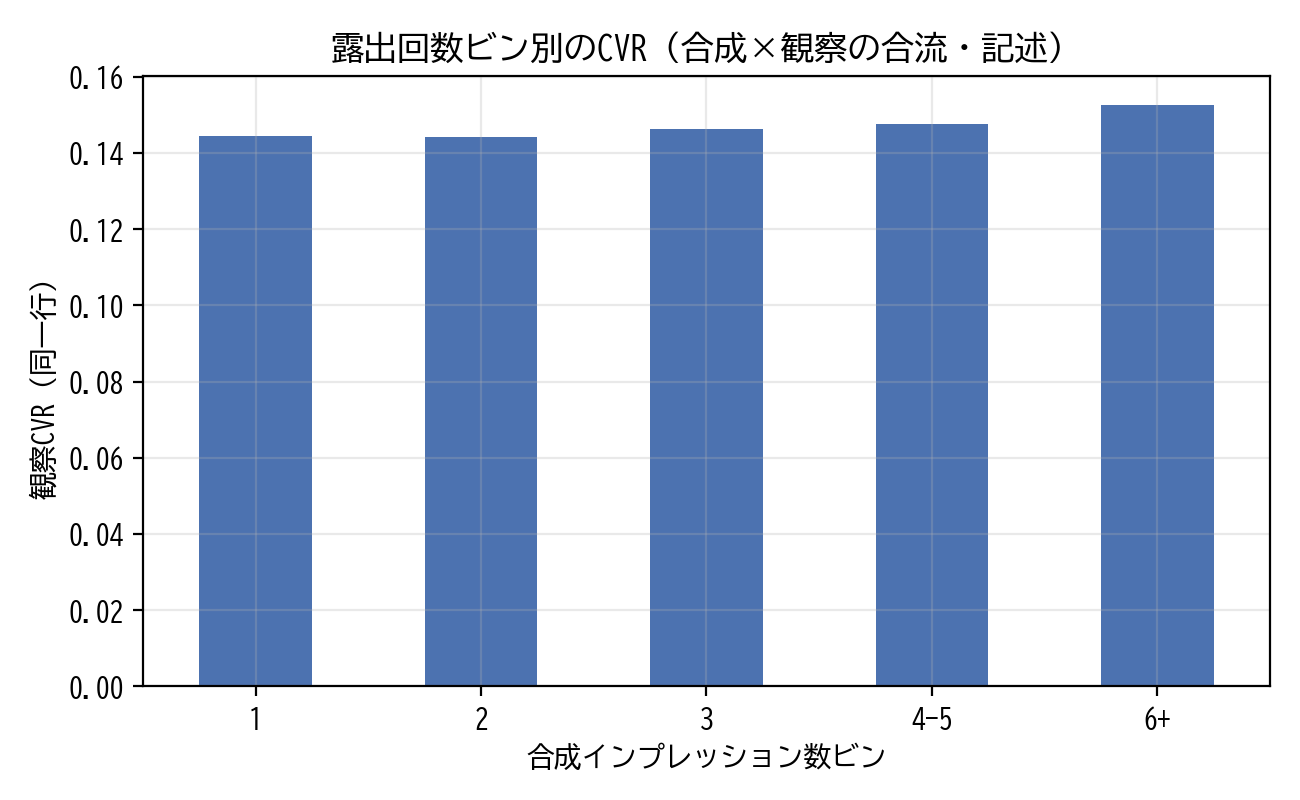
\includegraphics[width=\linewidth]{../figures/appendix/fig_cvr_by_impression_bin.png}
    \caption{インプレッション数ビン別の観察CVR（記述）。}
    \label{fig:app-cvr-imp}
  \end{subfigure}\hfill
  \begin{subfigure}[t]{0.49\linewidth}
    \centering
    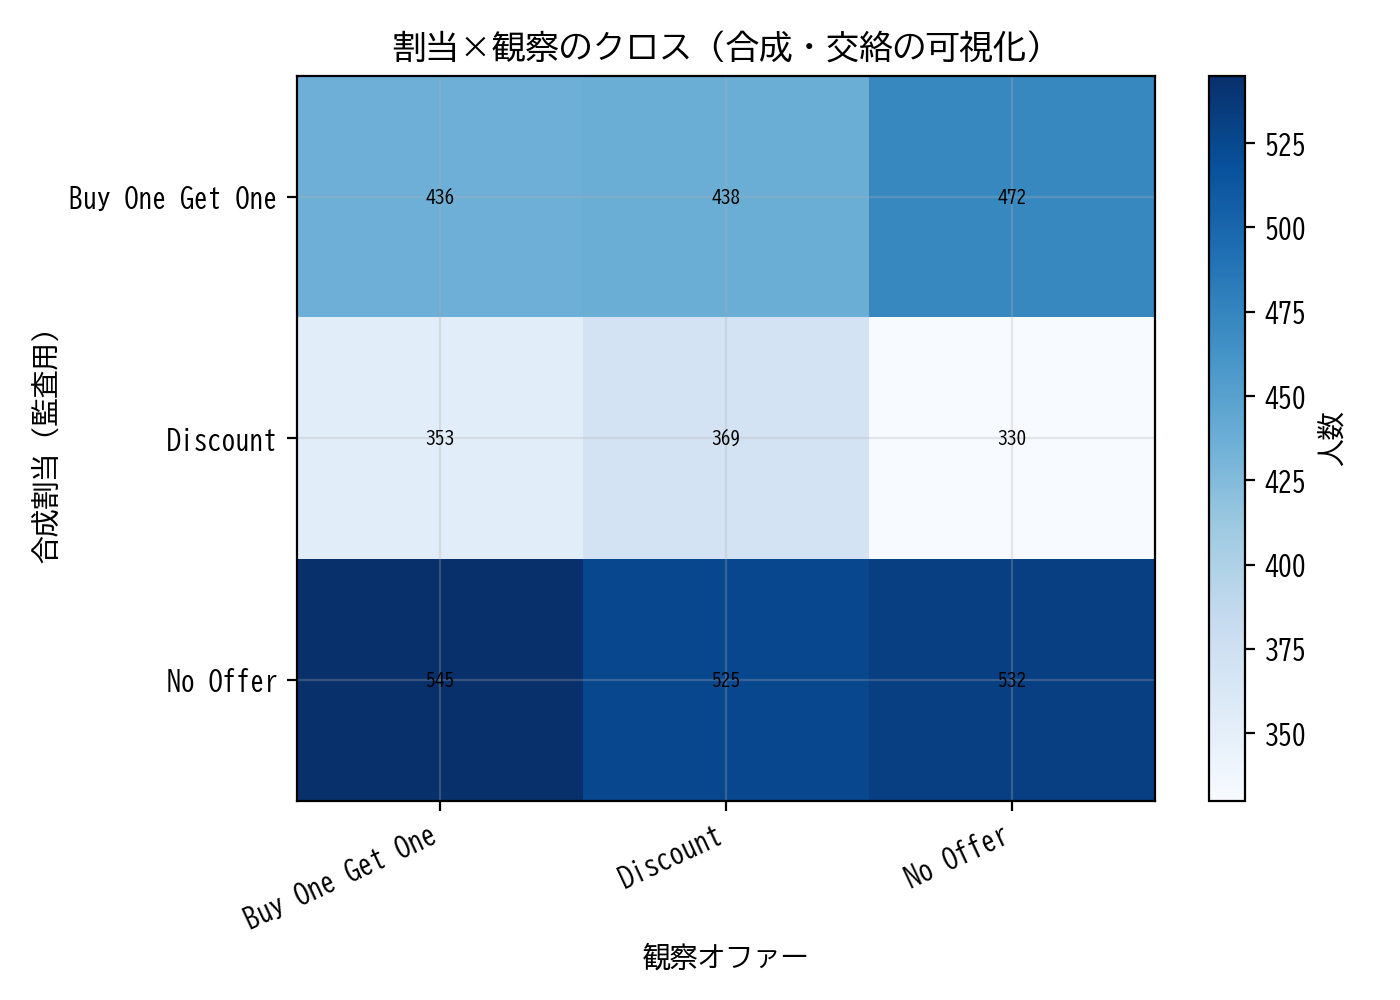
\includegraphics[width=\linewidth]{../figures/appendix/fig_assignment_cross_heatmap.png}
    \caption{合成割当と観察オファーのクロス。}
    \label{fig:app-assign-heat}
  \end{subfigure}
  \caption{合成ログに基づく記述（左：CVRビン、右：割当クロス）}
\end{figure}

\begin{figure}[!htbp]
  \centering
  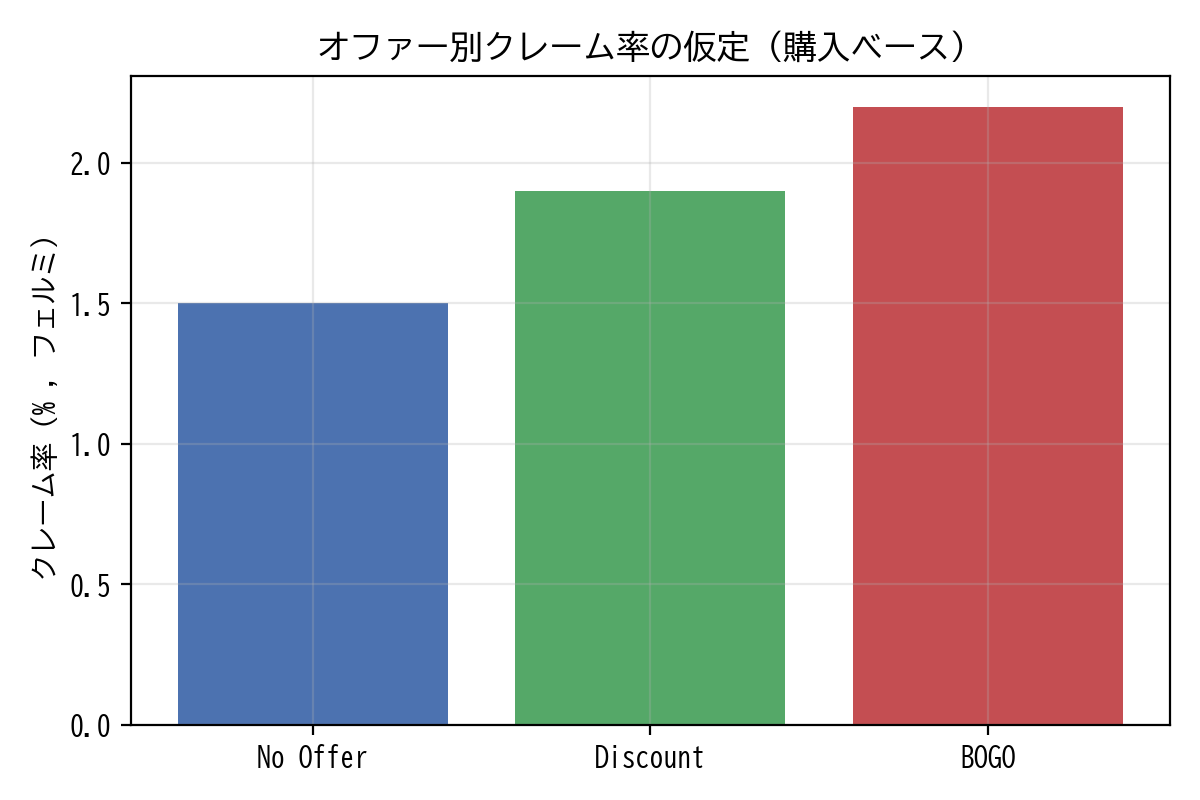
\includegraphics[width=0.92\linewidth]{../figures/appendix/fig_claims_rate_by_offer.png}
  \caption{オファー別クレーム率のフェルミ仮定。}
  \label{fig:app-claims}
\end{figure}

\begin{figure}[!htbp]
  \centering
  \begin{subfigure}[t]{0.49\linewidth}
    \centering
    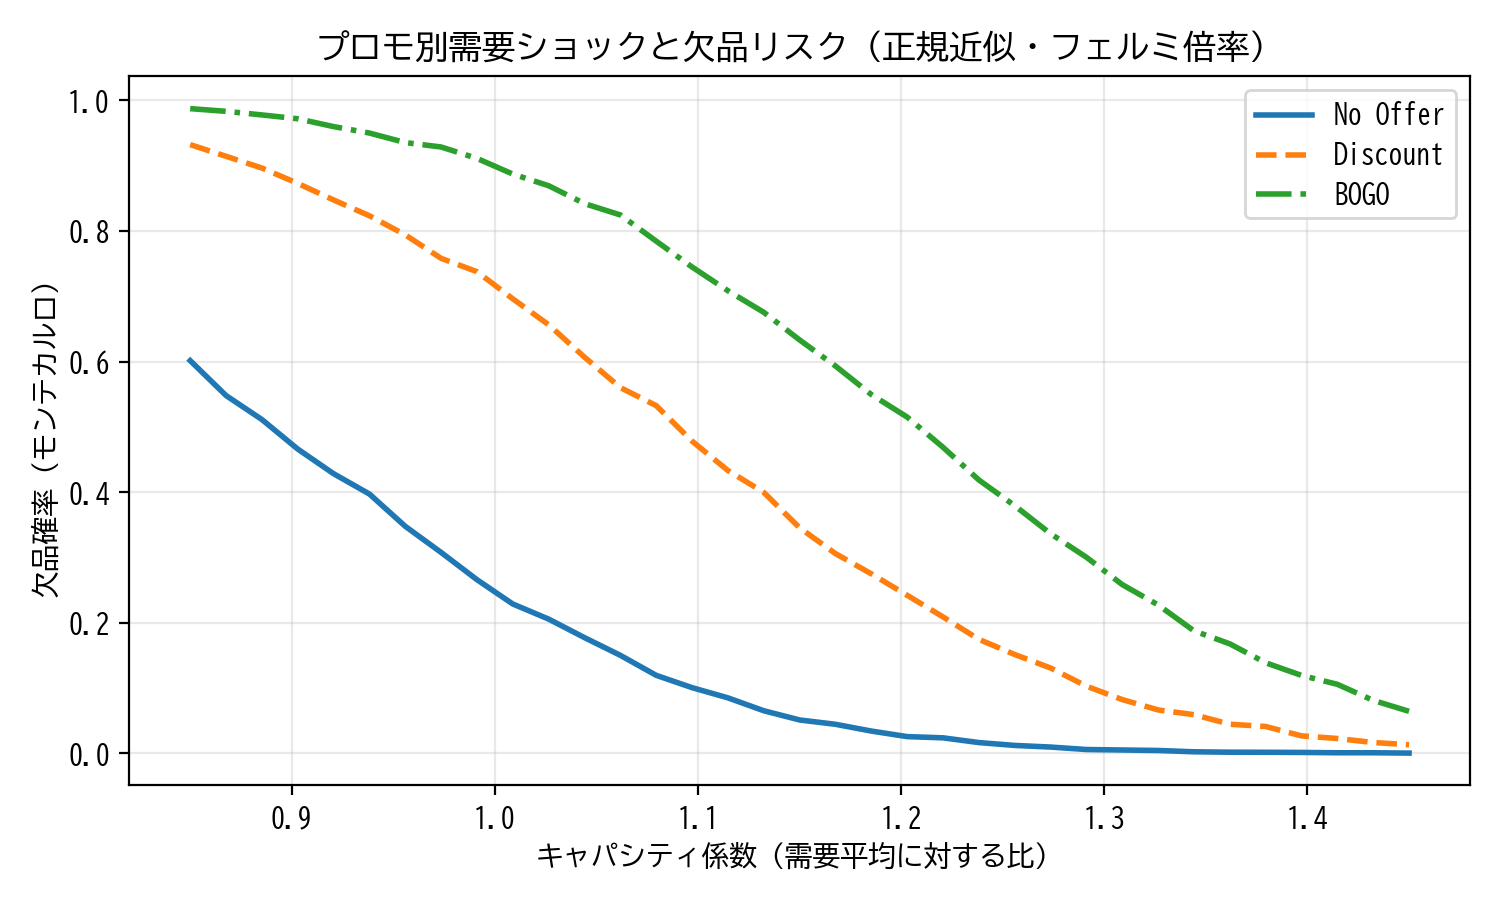
\includegraphics[width=\linewidth]{../figures/appendix/fig_inventory_stockout.png}
    \caption{需要ショックに対する欠品確率（モンテカルロ）。}
    \label{fig:app-inventory}
  \end{subfigure}\hfill
  \begin{subfigure}[t]{0.49\linewidth}
    \centering
    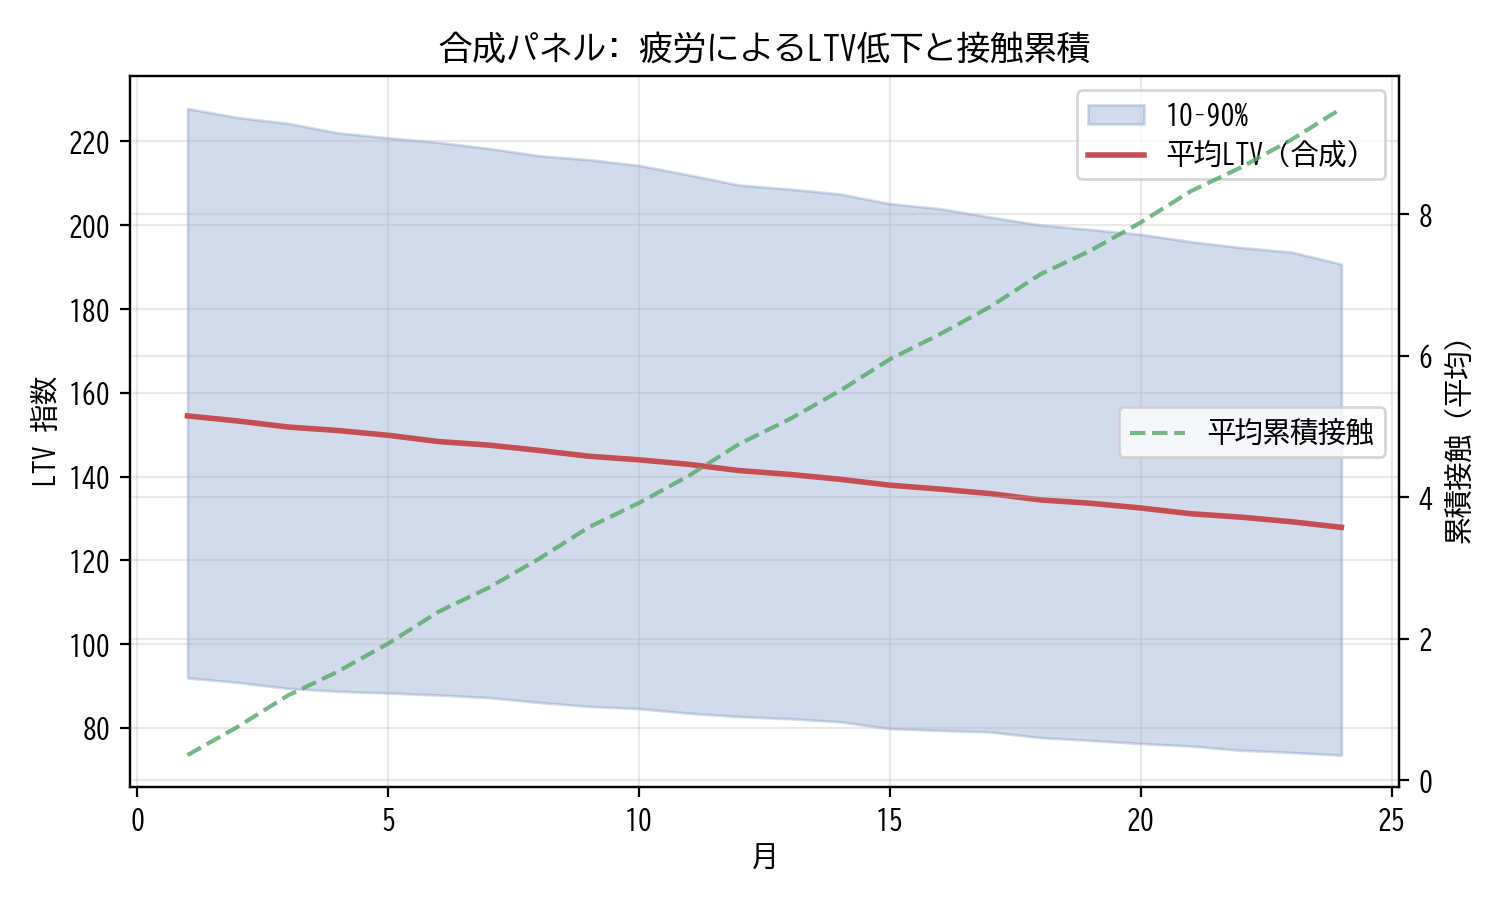
\includegraphics[width=\linewidth]{../figures/appendix/fig_panel_ltv_fatigue.png}
    \caption{合成パネル：LTVと累積接触（疲労）。}
    \label{fig:app-panel}
  \end{subfigure}
  \caption{在庫リスクと長期パネル（合成）}
\end{figure}

\begin{figure}[!htbp]
  \centering
  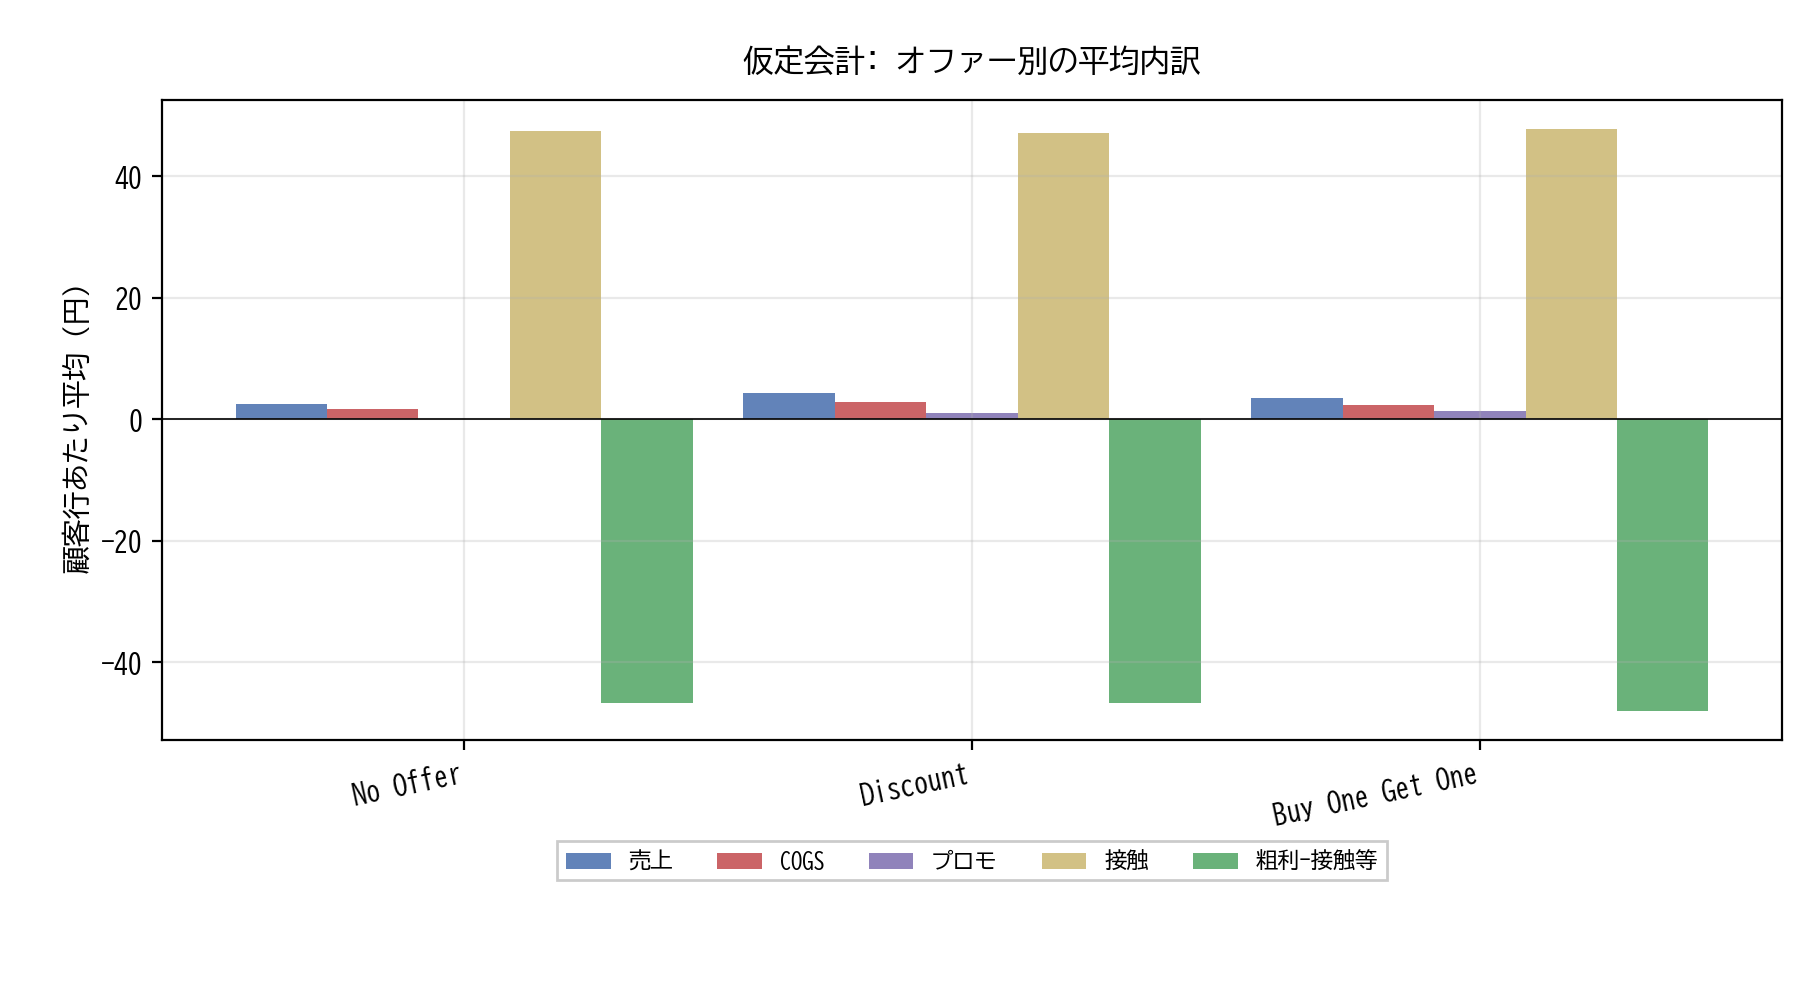
\includegraphics[width=0.92\linewidth]{../figures/appendix/fig_profit_components_grouped.png}
  \caption{仮定会計におけるオファー別の平均内訳（売上・COGS・プロモ・接触・粗利）。凡例は図内の棒グラフの下に配置。}
  \label{fig:app-profit-grouped}
\end{figure}
